\documentclass[10pt]{article}
\usepackage{graphicx} % Required for inserting images
\usepackage{xcolor}
% Tarih Ekleme
\usepackage[ddmmyyyy]{datetime}
\renewcommand{\dateseparator}{.}
\graphicspath{{./}}

\title{GAN ile Tümörlü Beyin MR Görüntüleri Oluşturma}
\author{Emre Akkaya}

\begin{document}
	
	\begin{figure}
		\centering
		
\includegraphics{ksbu.jpg}
	\end{figure}
	
	\maketitle
	
	\section*{Özet}
	Bu projede, beyin tümörlerinin erken teşhisinde önemli bir rol oynayan bir yapay zeka modeli geliştirilmesi amaçlanmıştır. Beyin tümörleri, sağlık endüstrisinde ciddi bir sağlık sorunu oluşturmaktadır ve erken teşhis, tedavi sürecindeki başarıyı büyük ölçüde etkilemektedir. Proje kapsamında Kaggle'dan alınan \textit{brain-tumor-dataset} veri seti kullanılmış ve proje içinde tümörlü resimlerden \textit{seed} değişkeni kullanılarak 10 adet eğitim verisi seçilip bunların eğitim işlemleri gerçekleştirilmiştir. Eğitim süreci tamamlandıktan sonra, modelin performansı dikkatle değerlendirilmiş ve gerektiğinde iyileştirmeler yapılmıştır. Yapılan testler sonucunda, geliştirilen modelin yeni tümörlü beyin görüntülerini başarıyla tespit edebildiği ve bu alanda literatüre önemli bir katkı sağladığı görülmüştür.
	
	\noindent \textbf{Anahtar Kelimeler:} Beyin Tümörü, MR Görüntüleri, Derin Öğrenme, GAN, Yapay Zeka, Tıbbi Görüntüleme
	
	\section{Giriş}
	Beyin tümörleri, dünya genelinde ciddi bir sağlık sorunu oluşturmaktadır. Erken teşhis, hastalığın tedavisinde kritik bir rol oynamaktadır. Geleneksel teşhis yöntemleri çoğunlukla zaman alıcı ve maliyetli olabilmektedir. Bu çalışmada, beyin tümörlerinin teşhisinde kullanılabilecek bir yapay zeka modeli geliştirilmesi amaçlanmıştır. Çalışmadaki motivasyonumuz, sağlık endüstrisinde önemli bir yere sahip olan tıbbi görüntüleme alanına yenilikçi bir katkı sağlamaktır. Beyin tümörlerinin erken teşhisi, hastaların tedavi süreçlerinde önemli bir avantaj sağlayacaktır. Bu çalışmaya başlama sebebimiz, mevcut yöntemlerin yetersizliği ve yapay zeka modellerinin bu alandaki potansiyel faydalarına duyduğumuz inançtır. Bu çalışmada, GAN (Generative Adversarial Network) kullanılarak yeni beyin tümörlü MR görüntüleri oluşturulmuştur. Önceki çalışmalarda, yapay zeka modellerinin tıbbi görüntülemede başarılı sonuçlar verdiği görülmüş, ancak çoğu çalışma yeterli veri seti bulunmaması nedeniyle sınırlı kalmıştır. Bu çalışmada, yeterli miktarda veri toplanarak modelin performansı artırılmıştır. Bu çalışma, beyin tümörlerinin teşhisinde yapay zeka kullanımına yeni bir bakış açısı getirmiştir. Modelin eğitimi için 155 adet tümörlü ve 98 adet tümörsüz MR görüntüsü kullanılmıştır.
	
	\section{Veri/Literatür Araştırması}
	Bu bölümde, çalışmada kullanılan veri seti ve deneysel çalışma düzenekleri hakkında detaylı bilgiler verilmiştir. Beyin MR görüntüleri, çeşitli görüntüleme teknikleri kullanılarak toplanmıştır. Veri seti, 155 adet tümörlü ve 98 adet tümörsüz MR görüntüsünden oluşmaktadır. Bu veriler, Google Drive üzerinden yüklenmiş ve ön işlemlerden geçirilmiştir. Görüntüler, 128x128 boyutlarına küçültülerek gri tonlamaya dönüştürülmüştür. GAN modeli, görüntülerin gerçekliğini artırmak ve daha yüksek kaliteli görüntüler oluşturmak amacıyla kullanılmıştır. Eğitim sürecinde, veri seti normalize edilerek modele sunulmuş ve çeşitli iyileştirmeler yapılmıştır.
	
	\section{Yöntem}
	Çalışmada, GAN modeli kullanılarak yeni beyin tümörlü MR görüntüleri oluşturulmuştur. GAN modeli, bir üretici (generator) ve bir ayrıştırıcı (discriminator) modelden oluşmaktadır. Üretici model, rastgele gürültüden gerçekçi görüntüler üretirken, ayrıştırıcı model bu görüntülerin gerçek mi yoksa sahte mi olduğunu ayırt etmeye çalışır. Üretici model, Transposed Convolution katmanları kullanarak rastgele gürültüden görüntüler üretir. Ayrıştırıcı model ise Convolutional Neural Network (CNN) kullanarak bu görüntüleri sınıflandırır. Eğitim sürecinde, üretici ve ayrıştırıcı modeller sırayla eğitilerek birbirlerini geliştirirler. Modelin performansı, gerçek ve sahte görüntülerin doğru sınıflandırılması ile ölçülmüştür. Eğitim sürecinde kullanılan optimizasyon teknikleri ve parametreler detaylı bir şekilde açıklanmıştır.
	
	\subsection{Üretici Model}
	Bu ağ rastgele gürültüyü girdi olarak alır ve veri (görüntüler gibi) üretir. Amacı gerçek verilere mümkün olduğunca yakın veriler üretmektir. 
	
	\subsection{Mimari}
	Mimari değişiklik gösterse de, pek çok popüler GAN'daki (DCGAN gibi) üreticiler, bir görüntü oluşturmak için gürültü vektörünün üst örneklemesine yardımcı olan, aktarılmış evrişimli katmanlar kullanılarak oluşturulur. Üretici genellikle aşağıdaki bileşenlerin dizisinden oluşur.
	
	\subsection{Giriş Katmanı}
	Üretici, genellikle normal veya düzgün bir dağılımdan örneklenen rastgele bir gürültü vektörünü alan bir giriş katmanıyla başlar.
	
	\subsection{Tamamen Bağlı  Katmanlar}
	Ağın başlarında, giriş gürültü vektörünü daha sonraki işlemler için uygun bir şekle dönüştürmek için tamamen bağlı katmanlar kullanılabilir.
	
	\subsection{Toplu Normalleştirme}
	Bu teknik genellikle  önceki katmanın çıktısını normalleştirerek öğrenmeyi stabilize etmek için katmanlar arasında kullanılır.
	\subsection{Aktivasyon Fonksiyonları}
	ReLU (Rectified Linear Unit) veya Leaky ReLU, jeneratördeki aktivasyon fonksiyonları için yaygın seçimlerdir. Bu fonksiyonlar, modelin doğrusal olmayan işlevler öğrenmesini sağlar ve karmaşık veriler üretmesini destekler.
	
	\subsection{Transpoze Etkileşim Katmanları}
	Bu katmanlar, jeneratörün temelini oluşturur. Önceki katmandan gelen girdiyi daha yüksek bir uzamsal boyuta örnekleyerek, evrişimli katmanların bir CNN'de yaptığının tam tersini yaparlar.
	
	\subsection{Katman Yeniden Şekillendirme}
	Bu katmanlar, verileri istenen çıktı formatına yeniden şekillendirmek için kullanılır.
	\subsection{Çıkış Katmanı}
	Son katman, genellikle oluşturulan verinin doğasına bağlı olarak tanh veya sigmoid aktivasyon fonksiyonunu kullanır. Görüntü üretimi için, genellikle bir tanh fonksiyonu kullanılarak normalleştirilmiş bir aralıktaki piksel değerlerinin çıktısı alınır.
	
	\subsection{Ayrıştırıcı Model }
	Bu ağ, girdi olarak gerçek verileri ve Üretici tarafından oluşturulan verileri alır ve ikisini birbirinden ayırmaya çalışır. Verilen verinin gerçek olma olasılığını verir. 
	
	\subsection{Mimari}
	Ayırıcının mimarisi genellikle geleneksel evrişimli sinir ağlarının (CNN'ler) mimarisini yansıtır, ancak bazı ayarlamalar vardır. Genellikle aşağıdaki bileşenlerin dizisinden oluşur.
	\subsection{Evrişimsel Katmanlar}
	Bu katmanlar görüntü verilerinin işlenmesinde temeldir. Giriş görüntülerinden özelliklerin çıkarılmasına yardımcı olurlar. Evrişim katmanlarının sayısı, verilerin karmaşıklığına bağlı olarak değişebilir.
	\subsection{Toplu Normalleştirme}
	Bu bazen girdiyi bir katmana normalleştirerek öğrenmeyi stabilize etmek için katmanlar arasında kullanılır.
	
	
	
	\subsection{Aktivasyon Fonksiyonları}
	Sızdıran ReLU, ayırıcıdaki aktivasyon fonksiyonları için yaygın bir seçimdir. Ünite aktif olmadığında küçük bir eğime izin verir ve bu da antrenman sırasında eğim akışının korunmasına yardımcı olabilir.
	
	\subsection{Havuz Katmanları}
	Bazı mimariler, giriş verilerinin uzamsal boyutlarını aşamalı olarak azaltmak için havuz oluşturma katmanlarını (maksimum havuzlama gibi) kullanır.
	
	\subsection{Tamamen Bağlı Katmanlar}
	Ağın sonunda, evrişimli katmanlar tarafından çıkarılan özellikleri işlemek için tamamen bağlı katmanlar kullanılır ve son çıktı katmanı elde edilir.
	
	
	\subsection{Çıkış Katmanı}
	Son katman tipik olarak bir olasılık değeri çıkışı sağlayan sigmoid aktivasyon fonksiyonuna sahip tek bir nörondur.
	\begin{figure}[htbp]
		\centering
		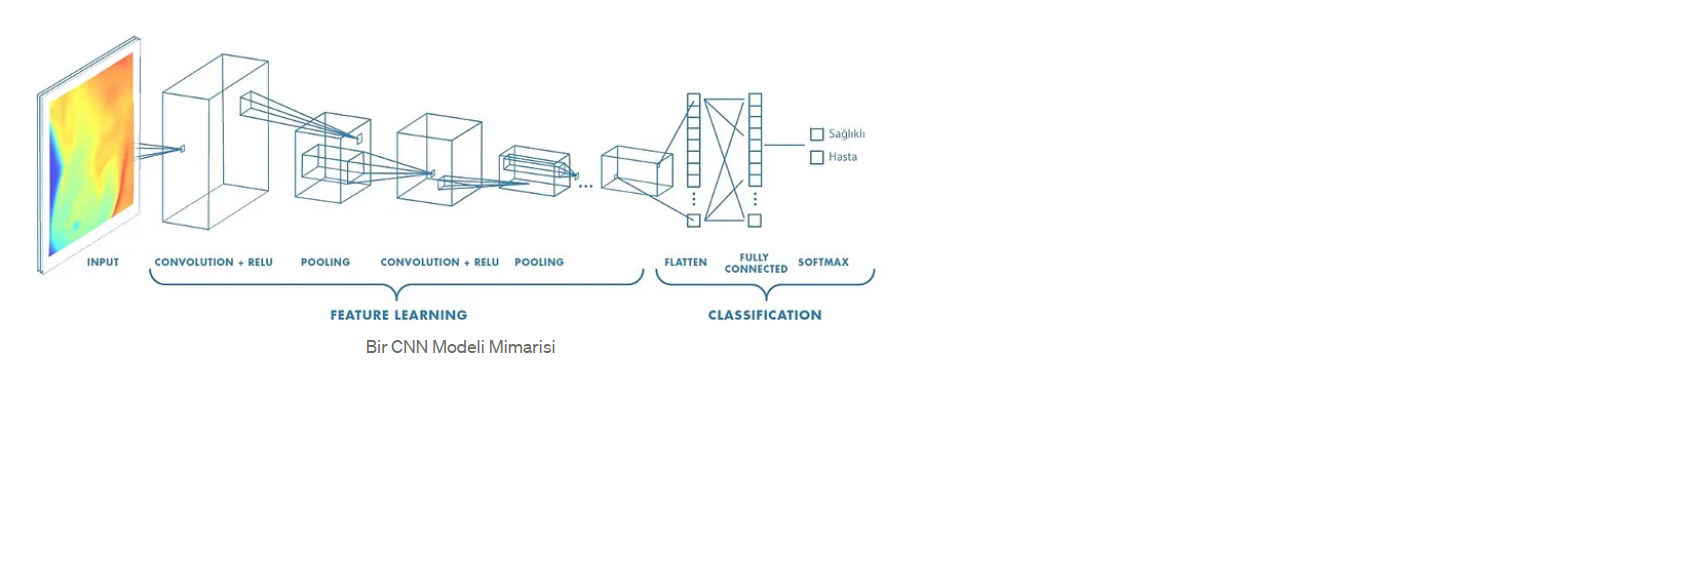
\includegraphics[width=0.8\linewidth]{mimari.png}
		\caption{Üretici ve Tüketici GAN Modeli \cite{kaggle}}
		\label{fig:uretici_tuketici}
	\end{figure}
	
	\subsection{Çalışma  Prensibi} 
	Eğitim sırasında Jeneratör, Discriminator'ın gerçek verilerden ayırt edemeyeceği verileri üretmeye çalışırken, Discriminator gerçek verileri sahte verilerden ayırma konusunda daha iyi olmaya çalışır. İki ağ özünde bir oyunda yarışıyor: Jeneratör ikna edici sahte veriler üretmeyi amaçlıyor ve Ayırıcı ise gerçeği sahteden ayırmayı amaçlıyor.
	
	
	
	
	\subsection{Üretici Model Oluşturulması } 
	Üretici model, gürültülü bir giriş alır ve bu girişi gerçek görüntüler gibi görünen yeni görüntülere dönüştürmek için transpoze konvolüsyon katmanları kullanır.
	buildgenerator fonksiyonunda, Sequential modeli kullanılarak bir üretici model oluşturuluyor.Modelde tamamen bağlı bir giriş katmanı (Dense) yer alıyor. Bu katman, gürültülü bir vektörü düzleştirmek ve ardından uygun boyutlara dönüştürmek için kullanılıyor.Ardından, Reshape katmanı ile giriş vektörü 3 boyutlu tensörlere dönüştürülüyor.Transpoze konvolüsyon katmanları (Conv2DTranspose) kullanılarak görüntü boyutları büyütülüyor ve özelliklerin daha karmaşık bir şekilde dönüştürülmesi sağlanıyor.Son olarak, çıkış katmanı, üretilen görüntüyü tanh aktivasyonu ile normalize ederek oluşturuyor.Model, binary cross-entropy kaybı ile ve Adam optimizasyon algoritması kullanılarak derleniyor.\cite{kaggle}
	
	
	\subsection{Ayrıştırıcı Model Oluşturulması}
	
	Ayrıştırıcı model, giriş olarak gerçek veya üretilmiş bir görüntü alır ve bu görüntünün gerçek veya sahte olduğunu sınıflandırır.	builddiscriminator fonksiyonu, yine Sequential modeli kullanarak bir ayrıştırıcı model oluşturuyor.
	Model, evrişimli katmanlar (Conv2D) ve tamamen bağlı katmanlar (Dense) içerir.
	Evrişimli katmanlar, özellik haritalarını çıkararak görüntüdeki özellikleri öğrenir.	Model, sigmoid aktivasyon fonksiyonu ile bir çıkış katmanı ile sonuçlanır, bu da gelen görüntünün gerçek veya sahte olduğunu belirler.
	Ayrıca, model binary cross-entropy kaybı ile ve Adam optimizasyon algoritması ile derlenir.\cite{kaggle}
	
	\subsection{Evrişimli Sistemler }
	Aktarılmış evrişim katmanlarını anlamak için önce normal evrişim katmanlarını anlamalıyız, çünkü paten kaymayı bilmeden buz hokeycisi olamayız.
	
	
	\subsection{Evrişimli Sinir Ağlarının Amacı}
	Kısaca bir girdiyi (genellikle görüntü)  bir çekirdek kullanarak alt örneklemektir
	
	\subsection{Evrişimli Sinir Ağlarının Önemi}
	CNN'ler, derin öğrenmede önemli bir ilerleme kaydetmiş ve özellikle görüntü sınıflandırma gibi görevlerde etkili olmuşlardır. İlk kullanımları 1990'larda karakter tanıma gibi görevlerde olmasına rağmen, Krizhevsky ve diğerleri tarafından 2012'de gerçekleştirilen ImageNet görüntü sınıflandırma yarışmasında büyük bir başarı elde edilmiştir.\cite{youtube}
	
	\subsection{Evrişimli Sinir Ağlarının Karmaşıklığı}
	Evrişimli sinir ağlarının kullanımı, özellikle ilk kez öğrenilirken karmaşık olabilir. Evrişimli katmanların çıkış şekli, girdinin şekli, çekirdek şekli, sıfır dolgu ve adımlar gibi faktörler tarafından etkilenir. Bu faktörler arasındaki ilişki kolayca anlaşılmaz ve tam olarak çıkarsanması zordur. Bununla birlikte, tamamen bağlı katmanlar, çıkış boyutunun girdi boyutundan bağımsız olduğu daha basit bir yapıya sahiptir. Ayrıca, CNN'ler genellikle havuzlama aşamasını içerir, bu da tamamen bağlı ağlara kıyasla daha fazla karmaşıklık ekler.\cite{youtube}
	
	
	
	\subsection{Evrişimli Sinir Ağları Nasıl Çalışır?}
	\begin{figure}[htbp]
		\centering
		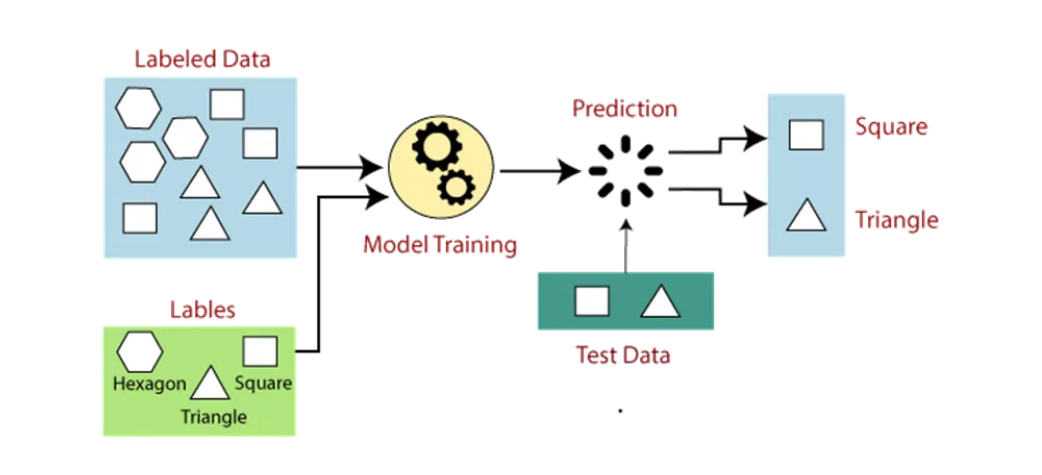
\includegraphics[width=0.7\linewidth]{resim1.png}
		\caption{ 2x2 lik alt örneklemenin 4x4 giriş üzerindeki adımları \cite{ytchannels}} 
		\label{fig:evrisim1}
	\end{figure}
	
	\begin{figure}[htbp]
		\centering
		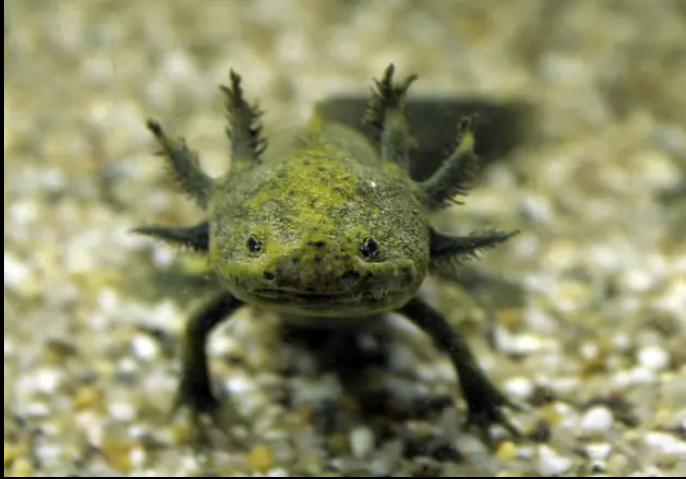
\includegraphics[width=0.7\linewidth]{resim2.png}
		\caption{3x3 lük çekirdek ve 4x4 lük giriş \cite{ytchannels}}
		\label{fig:evrisim2}
	\end{figure}
	
	\begin{figure}[htbp]
		\centering
		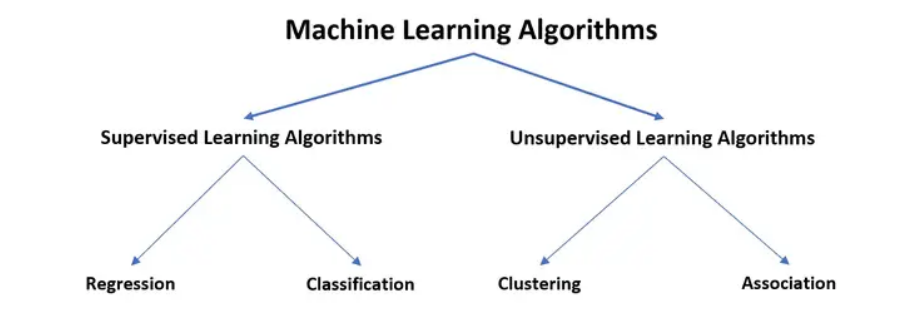
\includegraphics[width=0.7\linewidth]{resim3.png}
		\caption{Çekirdeğin ilk adımı \cite{ytchannels}}
		\label{fig:evrisim3}
	\end{figure}
	
	
	
	\begin{figure}[htbp]
		\centering
		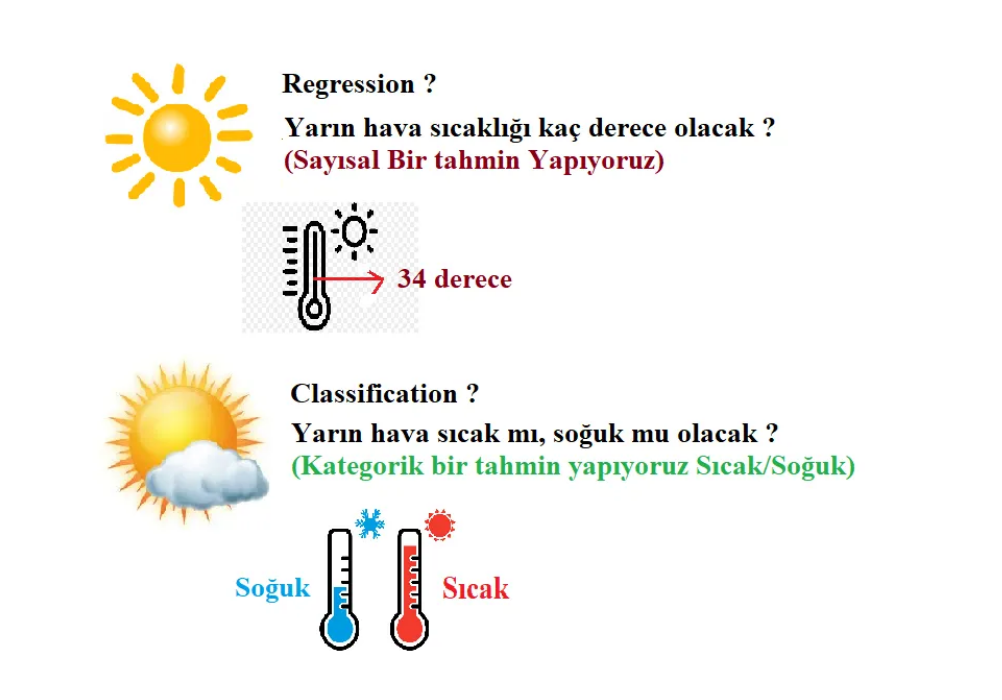
\includegraphics[width=0.7\linewidth]{resim4.png}
		\caption{Vektör haline getirilmiş c evrişimi \cite{ytchannels} }
		\label{fig:evrisim4}
	\end{figure}
	\begin{figure}[htbp]
		\centering
		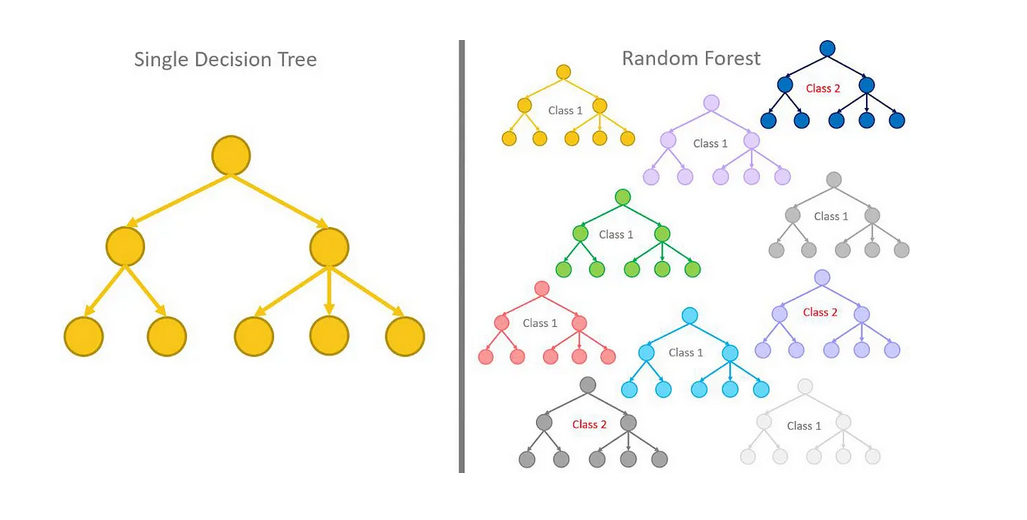
\includegraphics[width=0.7\linewidth]{resim5.png}
		\caption{Evrişimi vektörleştirme adımları \cite{ytchannels}}
		\label{fig:evrisim5}
	\end{figure}
	
	
	\begin{figure}[htbp]
		\centering
		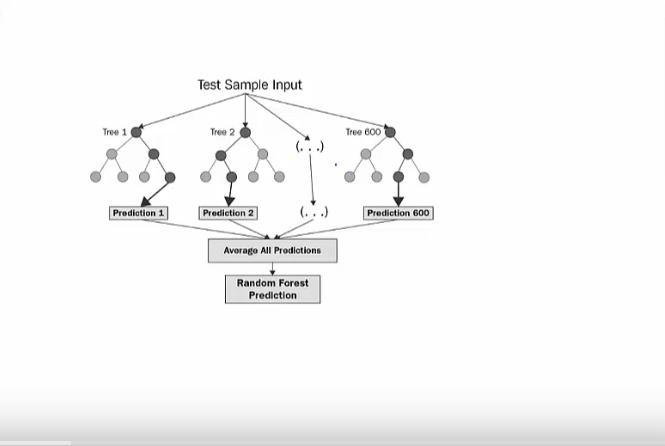
\includegraphics[width=0.7\linewidth]{resim6.png}
		\caption{Evrişimi vektörleştirme adımları \cite{ytchannels}}
		\label{fig:evrisim6}
	\end{figure}
	
	\begin{figure}[htbp]
		\centering
		\includegraphics[width=1.1\linewidth]{resim7.png}
		\caption{Evrişim formülü ve sonucu \cite{ytchannels}}
		\label{fig:evrisim7}
	\end{figure}
	
	
	
	\subsection{Aktarılmış Evrişimli Sistemler } 
	Transpoze etkileşim katmanları, evrişimli sinir ağlarında sıklıkla kullanılan bir tür katmandır. Bu katmanlar, genellikle evrişim (convolution) işleminin tersini gerçekleştirerek girdi boyutunu genişletirler. Evrişim katmanları, girdi verisinden özelliklerin çıkarılmasını sağlarken, transpoze etkileşim katmanları bu özellikleri tekrar orijinal boyuta döndürür. Bu nedenle, genellikle görüntü işleme ve yeniden oluşturma uygulamalarında kullanılırlar.
	Transpoze etkileşim katmanları, bir önceki evrişim katmanının çıktısını orijinal girdi boyutuna geri döndürmek için kullanılabilir. Örneğin, düşük çözünürlüklü bir görüntünün piksel değerlerini, yüksek çözünürlüklü bir görüntünün piksel değerlerine dönüştürmek için transpoze etkileşim katmanları kullanılabilir. Bu işlem, özellikle görüntü super resolution gibi uygulamalarda önemli bir rol oynar.
	Bu katmanlar, genellikle çekirdek boyutu ve adım (stride) gibi parametrelerle tanımlanır. Çekirdek, oluşturulacak her bir pikselin girdi görüntüsündeki hangi bölgeye karşılık geldiğini belirler. Ayrıca, sıfır dolgu (zero padding) ve aktivasyon fonksiyonları gibi ek parametrelerle birlikte kullanılarak çıktı boyutu ve detayı kontrol edilebilir.Aktarılmış evrişimli sistemlerde, genellikle bir evrişim (convolution) işleminin çıktısının daha sonra bir transpoze evrişim (transpose convolution) işlemine tabi tutulmasıyla elde edilir. Bu işlem, evrişim sonucunun giriş boyutuna uygun hale getirilmesini sağlar. Örneğin, 2x2'lik bir evrişim sonucunun girişe uygun 4x4 boyutunda bir çıktı elde etmek için bir transpoze evrişim işlemi uygulanabilir.
	
	\begin{figure}[htbp]
		\centering
		\includegraphics[trim={0 0 0 0},clip,width=1.35\linewidth]{resim9.png}
		\caption{Tranpoze Evrişim Oluşumu \cite{transposed_medium}}
		\label{fig:uretici_tuketici7}
	\end{figure}
	
	\begin{figure}[htbp]
		\centering
		\includegraphics[trim={0 0 0 0},clip,width=0.8\linewidth]{epoc1.jpg}
		\caption{Eğitim denemeleri sırasında Epoch 1' deki örnek görüntü }
		\label{fig:epoch1}
	\end{figure}
	
	\begin{figure}[htbp]
		\centering
		\includegraphics[trim={0 0 0 0},clip,width=0.8\linewidth]{epoc2.jpg}
		\caption{Eğitim denemeleri sırasında Epoch 50' deki  örnek görüntü }
		\label{fig:epoch1}
	\end{figure}
	
	
	
	
	
	
	
	\section{Bulgu ve Tartışma}
	Veri seti, toplamda 253 MR görüntüsünden oluşmaktadır. Görüntüler 128x128 piksel boyutunda ve gri tonlamalıdır. Eğitim sürecinde veri seti normalleştirilmiş ve modele sunulmuştur. Modelin eğitimi için başlangıçta 200 epoch kullanılmıştır. Modelde, üretici kısmında 3 transpoze katmanı, ayrıştırıcı kısmında ise 2 conv2d katmanı kullanılmıştır. Deneyler sonucunda modelin beyin tümörlerini başarıyla tespit edemediği ve modelin çöktüğü gözlemlenmiştir. Yaşanan bu durumun ardından, üretici modelde 2 transpoze katmanı ve 1 conv2d katmanı, ayrıştırıcıda ise 4 adet conv2d katmanı kullanılmıştır. Step-per-epoch sayısı 3750'ye çıkarılıp epoch sayısı 10'a düşürülmüştür. Böylece az ve daha güçlü adımlama ile sonuca ulaşılmaya çalışılmıştır. Ardından üretici tarafından üretilen görüntüler, ayrıştırıcı model tarafından doğru bir şekilde sınıflandırılmıştır. Modelin performansı, adım sayısının artırılması ve katmanların optimize edilmesi ile daha da iyileştirilmiştir. Eğitim sürecinde ayrıştırıcı ve üretici modellerin kayıpları (loss) düzenli olarak izlenmiş ve yeterince düşük olduğu görülmüştür. Sonuçlar, modelin yeni beyin tümörlerinin teşhisinde kullanılabilecek yeterlilikte olduğunu göstermektedir.
	
	
	
	\maketitle
	
	\subsection{Giriş }
	Oluşturduğum modeli eğittikten sonra 50 epoch sonunda oluşan görüntü aşağıdaki gibi oldu 
	
	\begin{figure}[htbp]
		\centering
		\includegraphics[width=0.428\linewidth]{epoc2.jpg}
		\caption{50. epoch sonundaki örnek görüntüler  }
		\label{fig:uretici_tuketici}
	\end{figure}
	
	\subsection{Veri Küçültme ve Çözünürlük Düşürme}
	Eğitim sonucunda oluşan görüntüler yeni beyin tümörleri tespit ediyor ancak resmin kalitesi gerçek verilere oldukça uzaktı bende veri setindeki resim sayısını azaltıp ardından çözünürlüğü de 64x64 yaptım .Eğitim süresi hızlı olsa da yüksek epochta bile görüntülerim kalitesiz oldu 
	
	
	
	\begin{figure}[htbp]
		\centering
		\includegraphics[width=0.428\linewidth]{resim23.jpg}
		\caption{Veri Azaltma ve Çözünürlük Düşürme sonucu 100. epoch sonundaki örnek görüntüler  }
		\label{fig:uretici_tuketici}
	\end{figure}
	
	\subsection{Gradyan Adım Sayısını Arttırma}
	Sorunu çözmek için bir başka yol denedim eğitim kodlarımda batch sizeyi 4 e düşürerek ve toplam adım sayısını her epoch için 3750 yaparak her epocthta çok ayrıntılı eğitim yapılmasını sağladım 
	\begin{figure}[htbp]
		\centering
		\includegraphics[width=0.428\linewidth]{resim24.png}
		\caption{Parametre Güncellemeleri   }
		\label{fig:uretici_tuketici}
	\end{figure}
	
	\subsection{Aşırı Uyum Sorunu}
	Eğitim sırasında 11.5 saat geçirdikten sonra modelim 8. epochta takıldı. Oluşturulan görüntüler gerçek verilere oldukça yakındı, ancak jeneratör her epochta benzer görüntüler üretmeye devam etti.
	\begin{figure}[htbp]
		\centering
		\includegraphics[width=0.85\linewidth]{resim18.png}
		\caption{Epoch 1 sonucu oluşan görüntü}
		\label{fig:uretici_tuketici}
	\end{figure}
	
	\begin{figure}[htbp]
		\centering
		\includegraphics[width=0.85\linewidth]{resim19.png}
		\caption{Epoch 2 sonucu oluşan görüntü}
		\label{fig:uretici_tuketici}
	\end{figure}
	
	\begin{figure}[htbp]
		\centering
		\includegraphics[width=0.85\linewidth]{resim20.png}
		\caption{Epoch 3 sonucu oluşan görüntü}
		\label{fig:uretici_tuketici}
	\end{figure}
	
	\begin{figure}[htbp]
		\centering
		\includegraphics[width=0.85\linewidth]{resim21.png}
		\caption{Epoch 4 sonucu oluşan görüntü}
		\label{fig:uretici_tuketici}
	\end{figure}
	
	\begin{figure}[htbp]
		\centering
		\includegraphics[width=0.85\linewidth]{resim17.png}
		\caption{Epoch 5 sonucu oluşan görüntü}
		\label{fig:uretici_tuketici}
	\end{figure}
	
	\clearpage % Sayfa kesme komutu
	
	\begin{figure}[htbp]
		\centering
		\includegraphics[width=0.85\linewidth]{resim22.png}
		\caption{Epoch 7 sonucu oluşan görüntü}
		\label{fig:uretici_tuketici}
	\end{figure}
	
	
	
	\subsection{GAN larda Mod Çöküşü}
	Mode collapse,  Üretken Rekabetçi Ağlarda (GAN'lar), jeneratör modelinin gerçek veri dağıtımının tüm çeşitliliğini yakalayamayan sınırlı sayıda çıktı ürettiği zaman ortaya çıkan bir olgudur\cite{gan_overfitting}.
	
	\subsection{GAN larda Mod Çöküşü Neden Önemli}
	GAN'lar yalnızca endüstrilerde değil aynı zamanda sağlık ve iklim bilimi gibi kritik sektörlerde de devrim yaratma potansiyeline sahiptir. Örneğin, araştırmacıların karmaşık iklim modellerini simüle etmek veya hastalık teşhisi için tıbbi görüntüleme oluşturmak için GAN'ları kullandığını hayal edin. Mod Çöküşü meydana gelirse, çeşitli simülasyonlar veya görüntüler yerine araştırmacılar tekrarlayan ve aynı çıktılarla sonuçlanır. Bu çeşitlilik eksikliği bilimsel ilerlemeyi ve yeniliği engelleyebilir\cite{gan_overfitting}.
	
	\subsection{GAN larda Mod Çöküşü Sebepleri}
	GAN'larda modun çökmesine çeşitli faktörler katkıda bulunur. Bunlardan biri Felaketsel Unutuştur. Bu olgu, belirli bir görev üzerinde eğitilen modelin, yeni bir görevi öğrenirken edindiği bilgileri unutması durumunu ifade eder. Modun çökmesinin bir diğer nedeni Ayırıcının Aşırı Uyumudur. Bu durum, eğitim süreci sırasında ayırıcının aşırı uyumu meydana gelirse, ayırıcı gerçek verileri oluşturulan verilerden ayırmada çok verimli hale gelebilir. Eğitim verilerinden belirli özellikleri veya karakteristikleri ezberleyebilir ve bu ezberlenen özelliklerle eşleşmeyen oluşturulan herhangi bir görüntüyü reddedebilir\cite{gan_overfitting}.
	
	\subsection{Modelde Yaptığım Değişiklikler: Modele Katman ve Dropout ekleme}
	Bu kısımda ayrıştırıcı modelime 2 adet transpoze katmanı ve Dropout fonksiyonunu ekleyerek gerçek ve sahte görüntüleri daha iyi ayırt etmesini ayrıca üreticinin daha iyi görüntü oluşturmasını sağladım. Dropout, yapay sinir ağlarının aşırı öğrenmesini (overfitting) önlemek için kullanılan bir düzenleme (regularization) tekniğidir. Bu teknik, eğitim sırasında her adımda rastgele olarak belirli oranlarda nöronları devre dışı bırakır. Örneğin, dropout(0.4) ifadesi, her eğitim adımında modelin nöronlarının yüzde kırkının rastgele olarak devre dışı bırakılacağını belirtir. Bu sayede model, yalnızca belirli nöronlara bağımlı kalmaz ve daha genelleştirilebilir özellikler öğrenir. Dropout oranını 0.4 olarak seçmemin nedeni, bu oranın modelin karmaşıklığını azaltarak daha iyi genel performans sağlamasıdır. Transpoze katmanlar ise, genellikle veri boyutunu artırarak daha detaylı ve yüksek çözünürlüklü görüntüler oluşturmak için kullanılır.
	
	\begin{figure}[htbp]
		\centering
		\includegraphics[width=0.6\linewidth]{eski_model}
		\caption{Önceki Model}
		\label{fig:eski_model}
	\end{figure}
	
	\begin{figure}[htbp]
		\centering
		\includegraphics[width=0.6\linewidth]{yeni_model}
		\caption{Yeni Model}
		\label{fig:yeni_model}
	\end{figure}
	
	\subsection{Hata Aldım}
	Yaptığım değişiklikler sonrası generator eğitimi satırında hata aldım ve çözmem çok zamanımı aldı.
	
	\begin{figure}[htbp]
		\centering
		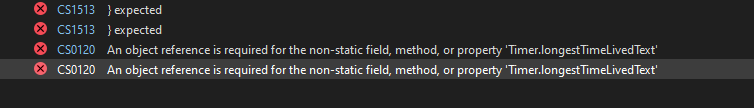
\includegraphics[width=0.8\linewidth]{hata.png}
		\caption{Alınan hata}
		\label{fig:hata}
	\end{figure}
	
	\begin{figure}[htbp]
		\centering
		\includegraphics[width=0.542\linewidth]{resim16.png}
		\caption{Optimizasyon Hatasını Konsolda Görme}
		\label{fig:hata_cozumu}
	\end{figure}
	
	\subsection{Hatayı Çözme}
	Hatayı çözmek için yaptığım araştırmalar sonucu optimizörü build etmem gerektiğini farkettim ve kodum çalıştı. 
	
	\begin{figure}[htbp]
		\centering
		\includegraphics[width=0.8\linewidth]{hata_cozumu.png}
		\caption{Hatayı Çözen Kod \cite{gan_hata}}
		\label{fig:hata_cozumu}
	\end{figure}
	
	\begin{itemize}
		\item \texttt{generator.trainable.variables}: Üretici modelin eğitilebilir (trainable) tüm değişkenlerini içerir.
		\item \texttt{discriminator.trainable.variables}: Ayrıştırıcı modelin eğitilebilir tüm değişkenlerini içerir.
	\end{itemize}
	
	Bu değişkenler, modelin ağırlıkları (weights) ve öngerilimleri (biases) gibi optimize edilecek parametrelerdir.
	
	\subsection{Bu İşlemin Amacı ve Önemi}
	\begin{itemize}
		\item \textbf{Modelin Tüm Parametrelerini Tanıtmak:} \texttt{optimizer.build()} fonksiyonu, optimizörün hangi değişkenleri optimize edeceğini belirler. Üretici ve ayrıştırıcı modellerin tüm eğitilebilir değişkenlerinin optimizöre tanıtılması, optimizasyon sürecinde bu değişkenlerin doğru bir şekilde güncellenmesini sağlar.
		\item \textbf{Model Eğitimi İçin Hazırlık:} Bu yapılandırma, eğitim süreci başlamadan önce optimizörün gerekli tüm bilgilere sahip olmasını sağlar. Bu adım, özellikle modellerin karmaşık ve büyük olduğu durumlarda önemlidir.
		\item \textbf{Uyumsuzluk ve Hataların Önlenmesi:} Tüm eğitilebilir değişkenlerin optimizöre tanıtılması, optimizasyon sürecinde ortaya çıkabilecek \texttt{KeyError} gibi hataların önlenmesine yardımcı olur. Böylece, optimizör tüm değişkenleri tanır ve güncelleme işlemlerini sorunsuz bir şekilde gerçekleştirir.
	\end{itemize}
	
	\subsection{Özet}
	Bu kod, Adam optimizörünü oluşturur ve bu optimizörü üretici ve ayrıştırıcı modellerin tüm eğitilebilir değişkenlerini optimize edecek şekilde yapılandırır. Bu, modelin doğru ve etkili bir şekilde eğitilmesi için önemli bir adımdır ve optimizasyon sürecinde ortaya çıkabilecek hataların önlenmesine yardımcı olur.
	
	
	
	
	\section{Sonuç}
	Bu çalışma ile beyin tümörlerinin teşhisinde kullanılabilecek bir yapay zeka modeli geliştirilmiştir. Model, GAN kullanılarak yeni ve gerçekçi beyin tümörlü MR görüntüleri üretmiş ve başarılı sonuçlar elde etmiştir. Çalışma, sağlık endüstrisinde tıbbi görüntüleme alanında önemli bir katkı sağlamaktadır. Gelecekte yapılması planlanan çalışmalar, daha büyük ve çeşitli veri setleri kullanılarak modelin performansını artırmak ve farklı türde tümörlerin tespitini mümkün kılmak olacaktır. Ayrıca, modelin klinik uygulamalarda kullanılabilirliğini artırmak için daha fazla test ve doğrulama çalışmaları yapılacaktır.
	
	
	
	\subsection{Yapılan Değişiklikler Sonucu oluşan Görüntüler}
	\begin{figure}[htbp]
		\centering
		\includegraphics[width=0.85\linewidth]{gan_epoc1.png}
		\caption{Epoch 1 sonucu oluşan görüntü}
		\label{fig:uretici_tuketici}
	\end{figure}
	
	\begin{figure}[htbp]
		\centering
		\includegraphics[width=0.85\linewidth]{gan_epoc2.png}
		\caption{Epoch 2 sonucu oluşan görüntü}
		\label{fig:uretici_tuketici}
	\end{figure}
	
	\begin{figure}[htbp]
		\centering
		\includegraphics[width=0.85\linewidth]{gan_epoc3.png}
		\caption{Epoch 3 sonucu oluşan görüntü}
		\label{fig:uretici_tuketici}
	\end{figure}
	
	\begin{figure}[htbp]
		\centering
		\includegraphics[width=0.85\linewidth]{gan_epoc4.png}
		\caption{Epoch 4 sonucu oluşan görüntü}
		\label{fig:uretici_tuketici}
	\end{figure}
	
	\begin{figure}[htbp]
		\centering
		\includegraphics[width=0.85\linewidth]{gan_epoc5.png}
		\caption{Epoch 5 sonucu oluşan görüntü}
		\label{fig:uretici_tuketici}
	\end{figure}
	
	\clearpage % Sayfa kesme komutu
	
	\begin{figure}[htbp]
		\centering
		\includegraphics[width=0.70\linewidth]{gan_epoc6.png}
		\caption{Epoch 6 sonucu oluşan görüntü}
		\label{fig:uretici_tuketici}
	\end{figure}
	
	\begin{figure}[htbp]
		\centering
		\includegraphics[width=0.70\linewidth]{gan_epoc7.png}
		\caption{Epoch 7 sonucu oluşan görüntü}
		\label{fig:uretici_tuketici}
		
	\end{figure}
	
	\begin{figure}[htbp]
		\centering
		\includegraphics[width=0.72\linewidth]{gan_epoc8.png}
		\caption{Epoch 8 sonucu oluşan görüntü}
		\label{fig:uretici_tuketici}
		
		
	\end{figure}
	
	\title{Generator ve Discriminator Kayıp Analizi}
	\author{Emre Akkaya}
	
	
	
	
	
	\maketitle
	
	\subsection{Discriminator Kaybı}
	Discriminator eğitilirken hem gerçek verileri hem de jeneratörden gelen sahte verileri sınıflandırır. Aşağıdaki işlevi en üst düzeye çıkararak, gerçek bir örneği sahte olarak veya sahte bir örneği (generator tarafından oluşturulan) gerçek olarak yanlış sınıflandırdığı için kendisini cezalandırır.
	
	\begin{figure}[htbp]
		\centering
		\includegraphics[width=0.7\linewidth]{dis_loss}
		\caption{Ayırıcı Kaybı Matematiksel Gösterimi}
		\label{fig:dis_loss}
	\end{figure}
	
	\begin{enumerate}
		\item \textbf{log(D(x))} Generatorün gerçek görüntüyü doğru şekilde sınıflandırma olasılığını ifade eder,
		\item \textbf{log(1-D(G(z)))} değerini maksimuma çıkarmak, generatorden gelen sahte görüntünün doğru şekilde etiketlenmesine yardımcı olacaktır \cite{loss_neptune}.
	\end{enumerate}
	
	\subsection{Discriminator Kayıp Değeri}
	\begin{itemize}
		\item \textbf{Düşük Discriminator Kaybı:} Discriminator kaybının düşük olması, discriminator'ın gerçek ve sahte verileri iyi bir şekilde ayırt edebildiğini gösterir. Bu durum genellikle discriminator'ın güçlü olduğunu ve görevini başarılı bir şekilde yerine getirdiğini belirtir.
		\item \textbf{Yüksek Discriminator Kaybı:} Discriminator kaybının yüksek olması, discriminator'ın sahte verileri gerçek verilerden ayırt etmekte zorlandığını gösterir. Bu durum, generator'ın discriminator'ı kandırmada başarılı olduğunu veya discriminator'ın yeterince iyi öğrenemediğini işaret eder \cite{loss_stackovervlof}.
	\end{itemize}
	
	\subsection{Generator Kaybı}
	Generator eğitilirken rastgele gürültüyü örnekler ve bu gürültüden bir çıktı üretir. Çıktı daha sonra ayırıcıdan geçer ve ayırıcının birini diğerinden ayırt etme yeteneğine bağlı olarak "Gerçek" veya "Sahte" olarak sınıflandırılır.
	Jeneratörün kaybı daha sonra ayrımcının sınıflandırmasına göre hesaplanır; ayrımcıyı başarılı bir şekilde kandırırsa ödüllendirilir, aksi takdirde cezalandırılır. Jeneratörü eğitmek için aşağıdaki denklem en aza indirilmiştir \cite{loss_neptune}.
	
	\begin{figure}[htbp]
		\centering
		\includegraphics[width=0.7\linewidth]{gen_loss}
		\caption{Üretici Kaybı Matematiksel Gösterimi}
		\label{fig:gen_loss}
	\end{figure}
	
	\subsection{Generator Kayıp Değeri}
	\begin{itemize}
		\item \textbf{Düşük Generator Kaybı:} Generator kaybının düşük olması, generator'ın ürettiği sahte verilerin discriminator tarafından gerçek olarak sınıflandırıldığını gösterir. Bu durum, generator'ın başarılı olduğunu ve yüksek kaliteli sahte veriler ürettiğini gösterir.
		\item \textbf{Yüksek Generator Kaybı:} Generator kaybının yüksek olması, generator'ın ürettiği sahte verilerin discriminator tarafından kolayca sahte olarak tanındığını gösterir. Bu durum, generator'ın başarısız olduğunu ve ürettiği verilerin düşük kaliteli olduğunu gösterir \cite{loss_stackovervlof}.
	\end{itemize}
	
	\subsection{Generator Kaybının Discriminatorden Fazla Olması}
	\begin{enumerate}
		\item \textbf{Ayırıcı'nın Daha Hızlı Öğrenmesi:} Discriminator (ayırt edici), sahte ve gerçek veriler arasındaki farkları öğrenmede genellikle daha hızlıdır çünkü bu model, yalnızca bir sınıflandırma problemine odaklanır. Bu nedenle discriminator kaybı genellikle daha hızlı bir şekilde azalır ve düşük seviyelerde kalır.
		\item \textbf{Üretici'nin Zorlu Görevi:} Generator (üretici) daha zor bir göreve sahiptir: Gerçek veriye benzeyen yeni örnekler oluşturmak. Bu, daha karmaşık bir optimizasyon problemidir ve generator'ın discriminator'ı kandırmayı öğrenmesi zaman alır. Bu nedenle generator kaybı genellikle daha yüksek kalır \cite{loss_stackovervlof}.
	\end{enumerate}
	
	\subsection{Kayıp Değerleri Grafiğe Dökmek}
	\begin{figure}[htbp]
		\centering
		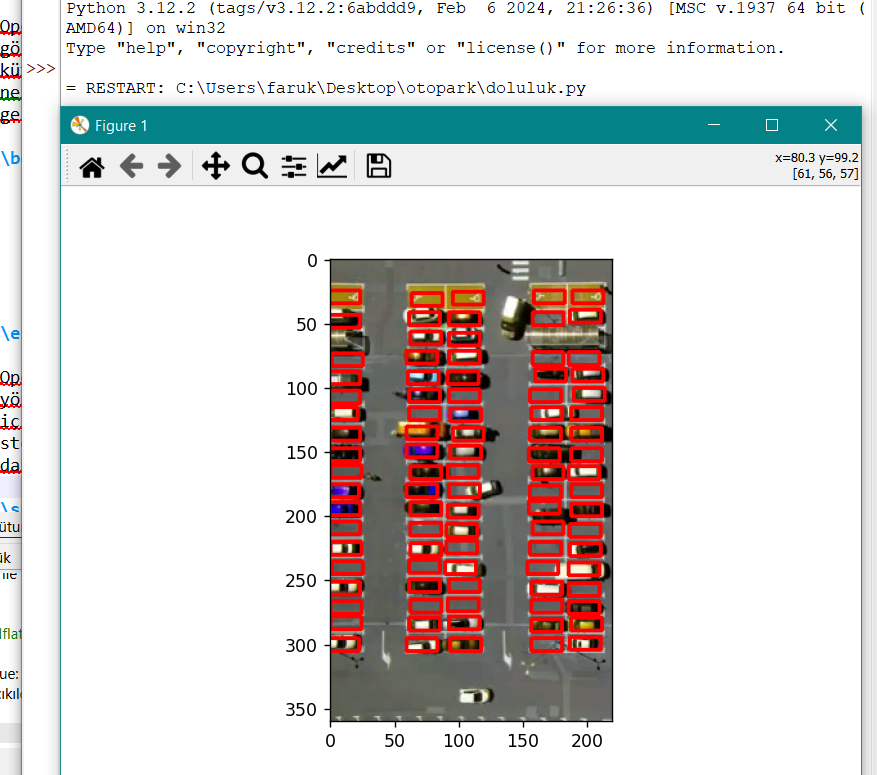
\includegraphics[width=0.5\linewidth]{plt}
		\caption{Kayıpları Grafiğe Aktarma Kodu}
		\label{fig:plt}
	\end{figure}
	
	\subsection{Kayıp Değer Grafiği}
	\begin{figure}[htbp]
		\centering
		\includegraphics[width=0.430\linewidth]{loss_grafik}
		\caption{Kayıpları Grafikte Görme}
		\label{fig:plt}
	\end{figure}
	
	\subsection{Grafik Analizi}
	\subsection{Discriminator Kayıp}
	\begin{itemize}
		\item[$\bullet$] İlk epoch'ta discriminator kaybı nispeten yüksek (0.026), ancak ikinci epoch'ta bu değer belirgin bir şekilde düşüyor (0.005).
		\item[$\bullet$] Sonraki epoch'larda kayıp değeri bir miktar dalgalanma gösterse de genellikle düşük kalıyor. Bu durum, discriminator'ın eğitim sürecinde nispeten istikrarlı bir şekilde performans gösterdiğini gösterir.
	\end{itemize}
	
	\subsection{Generator Kayıp}
	\begin{itemize}
		\item[$\bullet$] İlk epoch'ta generator kaybı oldukça yüksek (4.977), ardından ikinci epoch'ta daha da artıyor (8.451).
		\item[$\bullet$] Sonraki epoch'larda kayıp değerinde belirgin bir düşüş gözlemleniyor, ancak son epoch'ta yine bir artış görülüyor (8.500).
		\item[$\bullet$] Generator kayıpları daha dalgalı bir seyir izliyor, bu da generator'un discriminator tarafından daha iyi yakalanan sahte örnekler ürettiğini ve bu yüzden daha çok hata yaptığını gösterir.
	\end{itemize}
	
	
	
	
	
	
	
	
	
	
	
	\bibliographystyle{ieeetr}
	\bibliography{referans}
	
\end{document}
